\subsection{Twitter}
\begin{frame}[t]\frametitle{Twitter}

\begin{block}{Qué es Twitter}
    \begin{itemize}
        \item Red social creada en el 2006
        \item Usuarios variados: personas, instituciones gubernamentales, ONG, etc.
        \item Cada usuario puede escribir tuits con una longitud máxima de 140 carácteres{\footnote{Recientemente han aumentado el límite a 280 carácteres.}}
        \item \alert{Todos los tuits son públicos}
    \end{itemize}
\end{block}

\begin{block}{Porqué Twitter}
    \begin{itemize}
        \item Provee una interfaz pública para obtener tuits de cualquier persona
        \item Tópicos muy variados (gran diferencia con portales de noticias, por ejemplo)
        \item Escalabilidad
    \end{itemize}
    
\end{block}


\end{frame}

\subsection{Búsquedas geolocalizadas}



\begin{frame}[t]\frametitle{Búsquedas geolocalizadas}

La búsqueda geolocalizada es una herramienta que nos da la posibilidad de obtener tuits generados en un área geográfica particular. 
% Para esto, primero intenta buscar tuits cuyas coordenadas sean las buscadas.


\begin{columns}
    \begin{column}{0.30\textwidth}
        \begin{figure}
            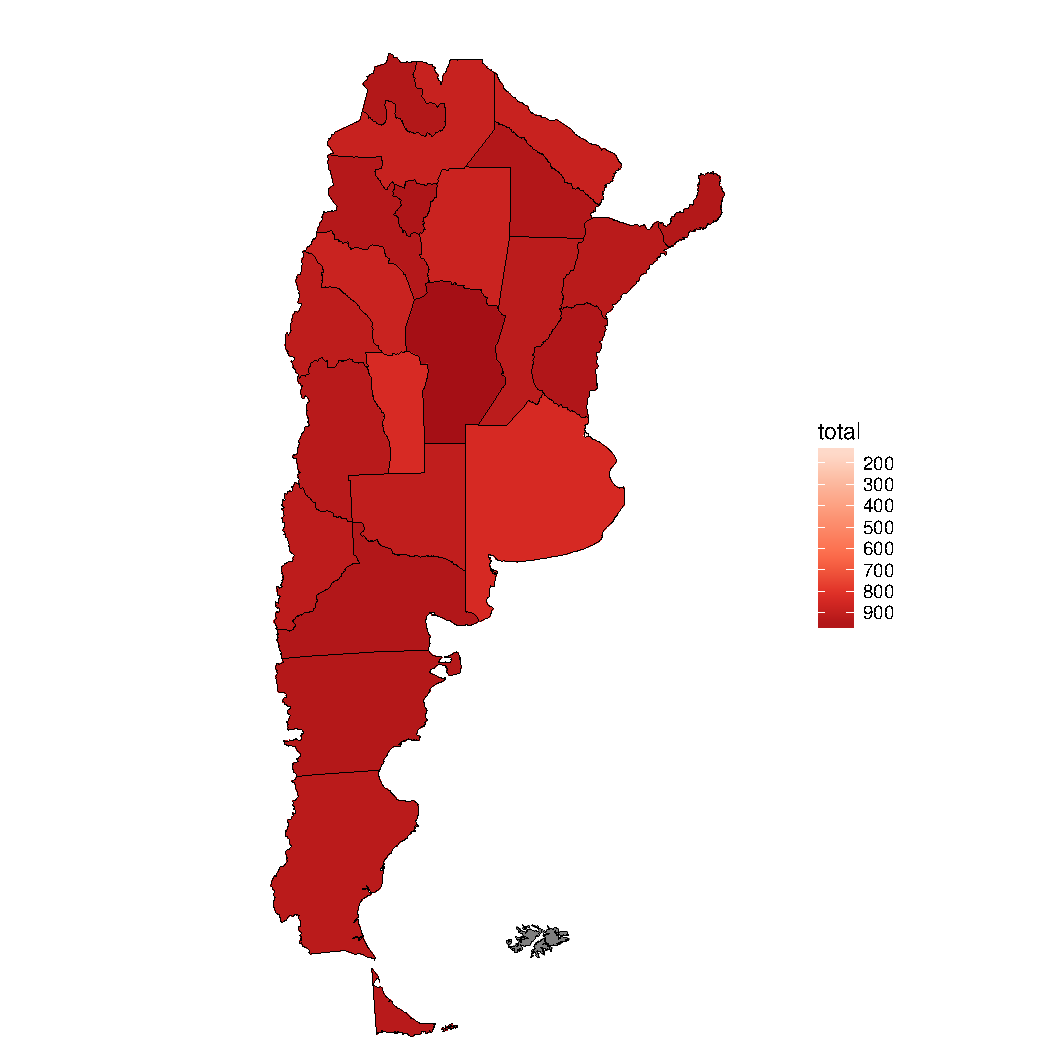
\includegraphics[width=\linewidth]{../src/images/mapaprovincias.pdf}
            % \caption{} 
            \label{fig:mapaProvincias}
        \end{figure}
    \end{column}

    \begin{column}{0.30\textwidth}
        \begin{figure}
            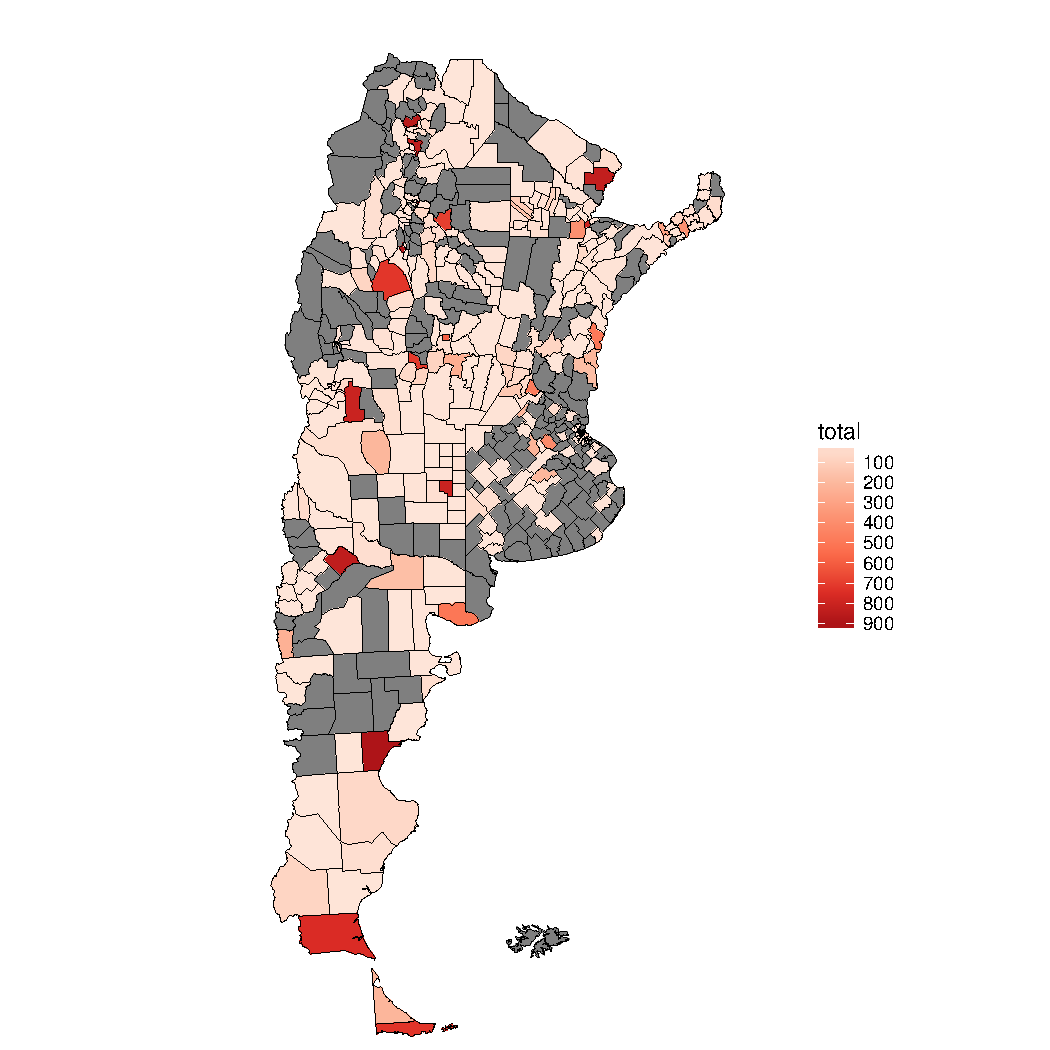
\includegraphics[width=\linewidth]{../src/images/mapadepartamentos.pdf}
            % \caption{} 
            \label{fig:mapaDepartamentos}
        \end{figure}
    \end{column}

    \begin{column}{0.30\textwidth}
        \begin{figure}
            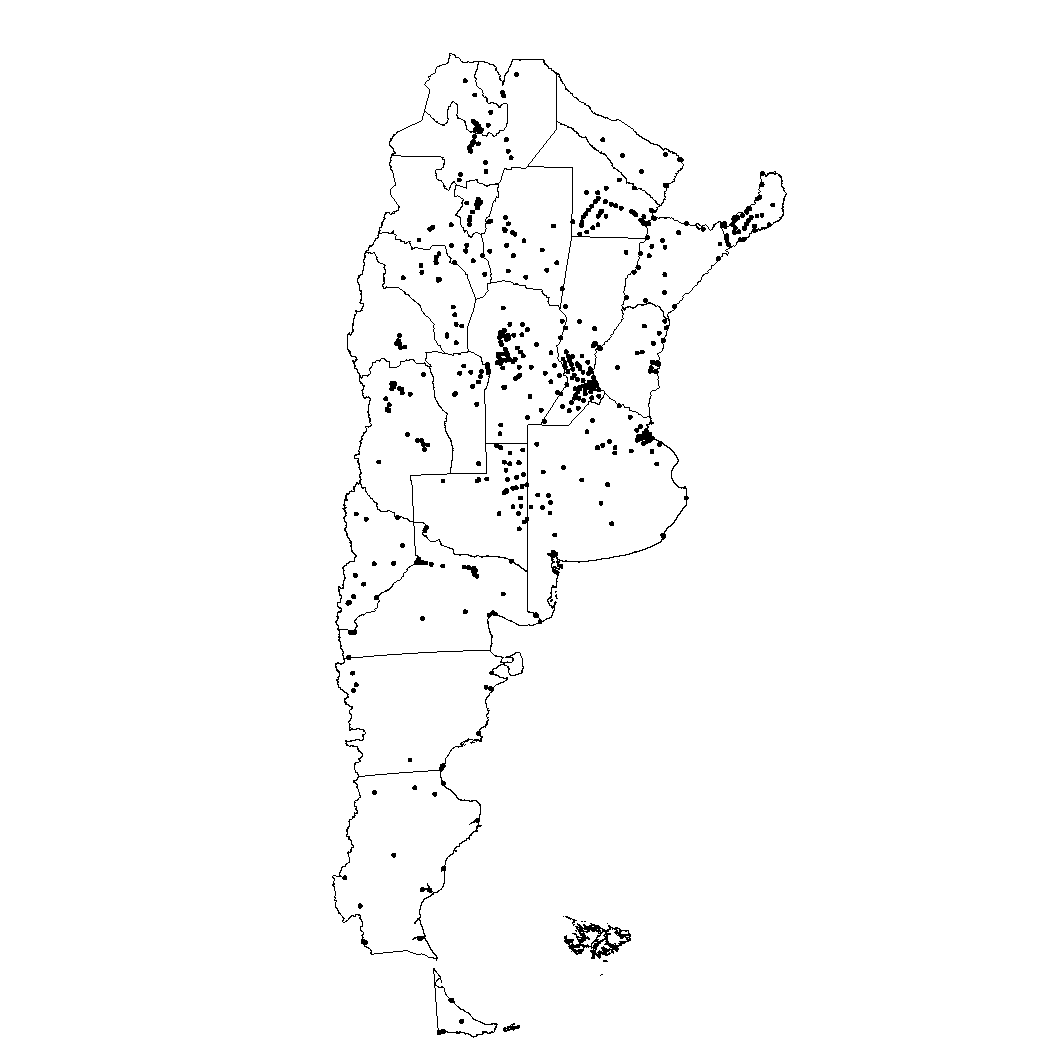
\includegraphics[width=\linewidth]{../src/images/mapaprovinciasConPuntos.pdf}
            % \caption{} 
            \label{fig:mapaPuntos}
        \end{figure}
    \end{column}
\end{columns}

\begin{itemize}
    \item Se realizaron búsquedas en todos los departamentos de las provincias argentinas.
    \item Nos quedamos con los usuarios que tienen como campo \textit{location} al menos uno de los nombres de las ciudades de la provincia. 

\end{itemize}



\end{frame}

\begin{frame}[t]\frametitle{Distribución temporal de tuits}
    ¿Y si en un momento dado la mayoría de los usuarios hablan del mismo tema por un fenómeno particular?
     \begin{columns}
    \only<2>{

    \begin{column}{.30\textwidth}
        \begin{figure}
        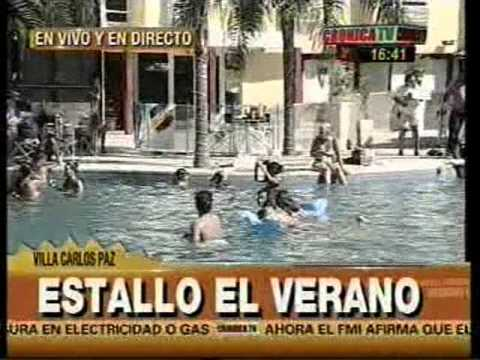
\includegraphics[width=0.9\textwidth]{../src/images/presentacion/estalloelverano.jpg}
        % \caption{} 
        \label{fig:estalloelverano}
        \end{figure}
    \end{column}

    \begin{column}{.30\textwidth}   
        \begin{figure}
        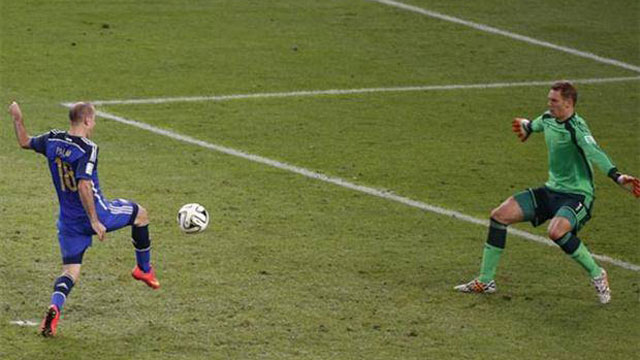
\includegraphics[width=0.9\textwidth]{../src/images/presentacion/eraporabajo.jpg}
        % \caption{} 
        \label{fig:eraporabajo}
        \end{figure} 
    \end{column}
    }
        
    \end{columns}
\only<3>{
\begin{figure}[!ht]\centering
   \begin{subfigure}[t]{0.42\textwidth}
     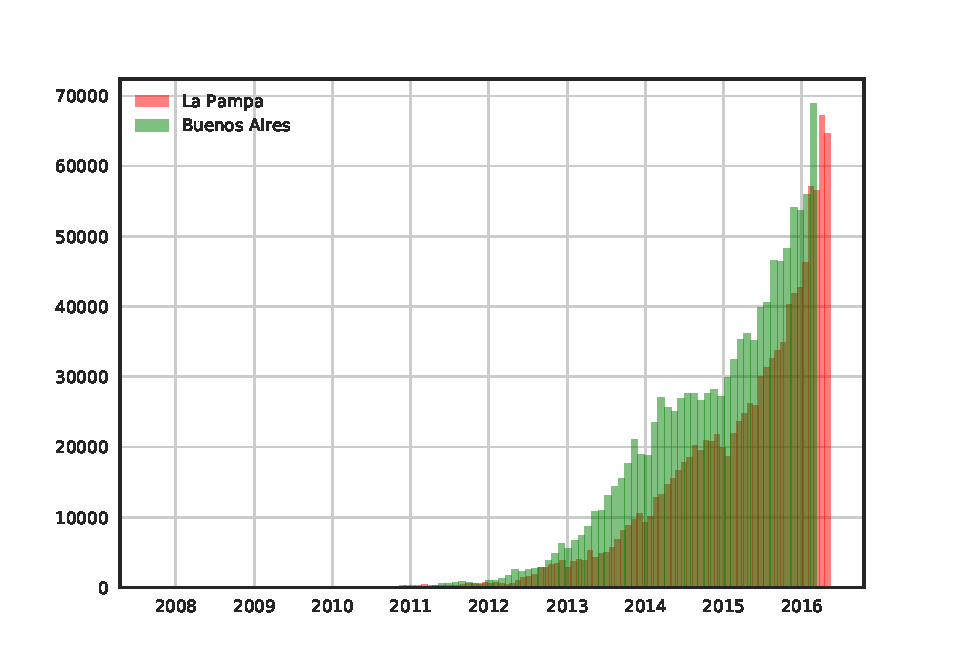
\includegraphics[width=\linewidth]{../src/images2/histTweetsProvincia1_sinFiltro.pdf}
     \phantomsubcaption
     \label{fig:histTweetsProvincia1}
   \end{subfigure}%
   \begin{subfigure}[t]{0.42\textwidth}
     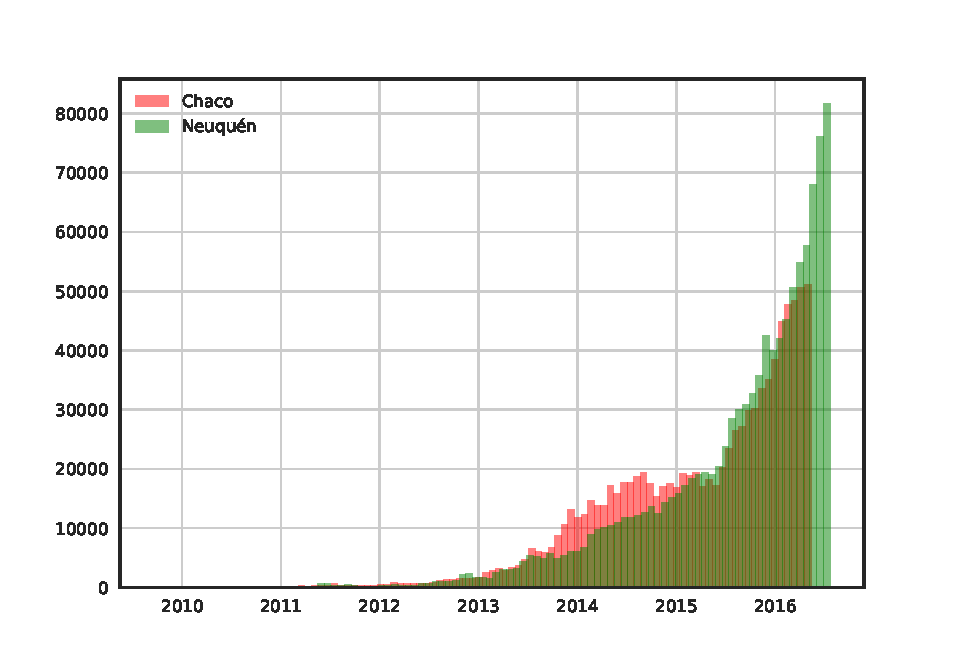
\includegraphics[width=\linewidth]{../src/images2/histTweetsProvincia2_sinFiltro.pdf}
     \phantomsubcaption
     \label{fig:histTweetsProvincia2}
   \end{subfigure}
    \caption{ \subref{fig:histTweetsProvincia1} Histograma de la cantidad de tuits que se hicieron por intervalo de tiempo en la provincias La Pampa y Buenos Aires. \subref{fig:histTweetsProvincia2} Gráfico para Chaco y Neuquén.}
   \label{fig:histTweets}
\end{figure}
}
    

\end{frame}

\begin{frame}[t]\frametitle{Balanceo de cantidad de tuits y de usuarios}
    
    \begin{table}
\centering
\scalebox{0.6}{
\begin{tabular}{|l|c|c|c|c|c|c|}
\hline
Provincia      & \#Palabras Distintas & \#Usuarios & \#Tuits & \#Total Palabras \\ \hline
Buenos Aires   & 191919       & 920          & 1125042    & 8974372  \\
Catamarca      & 173104       & 957          & 1057019    & 8161309   \\
Chaco          & 169476       & 964          & 976943     & 7605991   \\
Chubut         & 182592       & 954          & 1023373    & 8884745   \\
Córdoba        & 207307       & 987          & 1224266    & 10075932  \\
Corrientes     & 183292       & 939          & 1044951    & 8426940   \\
Entre Ríos     & 188679       & 969          & 1193693    & 9462986  \\
Formosa        & 169254       & 903          & 923352     & 7184382   \\
Jujuy          & 171064       & 971          & 678004     & 5951778   \\
La Pampa       & 186593       & 935          & 1085757    & 8996318  \\
La Rioja       & 186041       & 946          & 704044     & 6757277  \\
Mendoza        & 193708       & 945          & 1099717    & 9402399   \\
Misiones       & 168400       & 972          & 984218     & 7790197   \\
Neuquén        & 188038       & 927          & 1111201    & 9021449   \\
Río Negro      & 194383       & 965          & 1215361    & 9991831  \\
Salta          & 188402       & 884          & 830916     & 7506652   \\
San Juan       & 183546       & 926          & 1002322    & 8377792  \\
San Luis       & 164185       & 896          & 1006464    & 8327093  \\
Santa Cruz     & 174089       & 935          & 876621     & 7432923  \\
Santa Fe       & 201879       & 937          & 1019620    & 8862328  \\
S. del Estero       & 166540       & 887          & 944109     & 7355729  \\
T. del Fuego & 197273       & 964          & 976426     & 8559218   \\
Tucumán        & 195643       & 962          & 1093874    & 9238526 \\
  \hline
\end{tabular}}
\caption{Cantidades del conjunto de datos}
\label{tab:cantidades}

\end{table}


\end{frame}

\subsection{Tokenización y normalización}

\begin{frame}[t]\frametitle{¿Qué es una palabra?}
    \begin{block}{Tokenización}
    Se consideró una palabra a las secuencias de caracteres formados únicamente por letras. Por lo tanto se eliminaron las menciones con @, los hashtags y links entre otros. Decidimos ignorar estos términos ya que no tienen interés lingüístico y agregarían mucho ruido a los datos.
    \end{block}

    \begin{block}{Normalización}
    Todas las letras se convirtieron a letra minúscula y las palabras con más de tres letras iguales de forma consecutiva se redujeron para que solo tengan tres repeticiones. De esta forma, el término \textit{padreeeee} y \textit{padreeee} fueron reducidos a una única unidad léxica (\textit{padreee}). Esto se hizo con la librería \textit{TweetTokenizer de NLTK}. 
    \end{block}

\end{frame}
